 The production of multijets through QCD processes has a huge cross section. On the other hand, only a small fraction of these events mimics the lepton+jets final state of the applied event selection and the selection efficiency for QCD multijet events is therefore tiny. The combination of huge cross section and tiny selection efficiency would require the generation of extremely large MC samples for this process in order to produce sufficient events that survive the event selection to guarantee a proper QCD modelling with decent statistics in the signal region.
 An alternative way of modelling QCD is to define sideband regions in data that are enriched in QCD events and take the distributions of the relevant kinematic variables directly from these data. In the following subsections we describe the definition of the QCD enriched sideband regions and the estimation of the QCD contribution to the signal region by means of a fit to a discriminiating variable. As the number of available events is larger in the 2J0T control region, we use this region for a proof of concept and detailed studies of the method which is then applied to the 2J1T region.

 
\subsection{Modelling of the QCD background in 2J0T}

The 2J0T control region is dominated by \QCD and W+light flavour jets events. The fraction of \QCD events can be significantly increased by inverting the isolation criterion for the muon ($\murelIso > 0.12$) in the 2J0T region. Figure~\ref{fig:qcdshape} shows for the transverse mass of the W boson a comparison between simulated QCD events in the isolated region ($\murelIso < 0.06$), in the anti-isolated region ($\murelIso > 0.12$), and in an intermediate region ($0.06 < \murelIso < 0.12$). Good agreement in the shapes of the distributions from the three orthogonal regions is found. Using samples of simulated events from all relevant signal and background processes the \QCD-purity of the anti-isolated  sideband region has been estimated to be 95\%. Therefore the small contributions from non-\QCD-processes can be neglected. 

\begin{figure}[hbpt]
\begin{center}
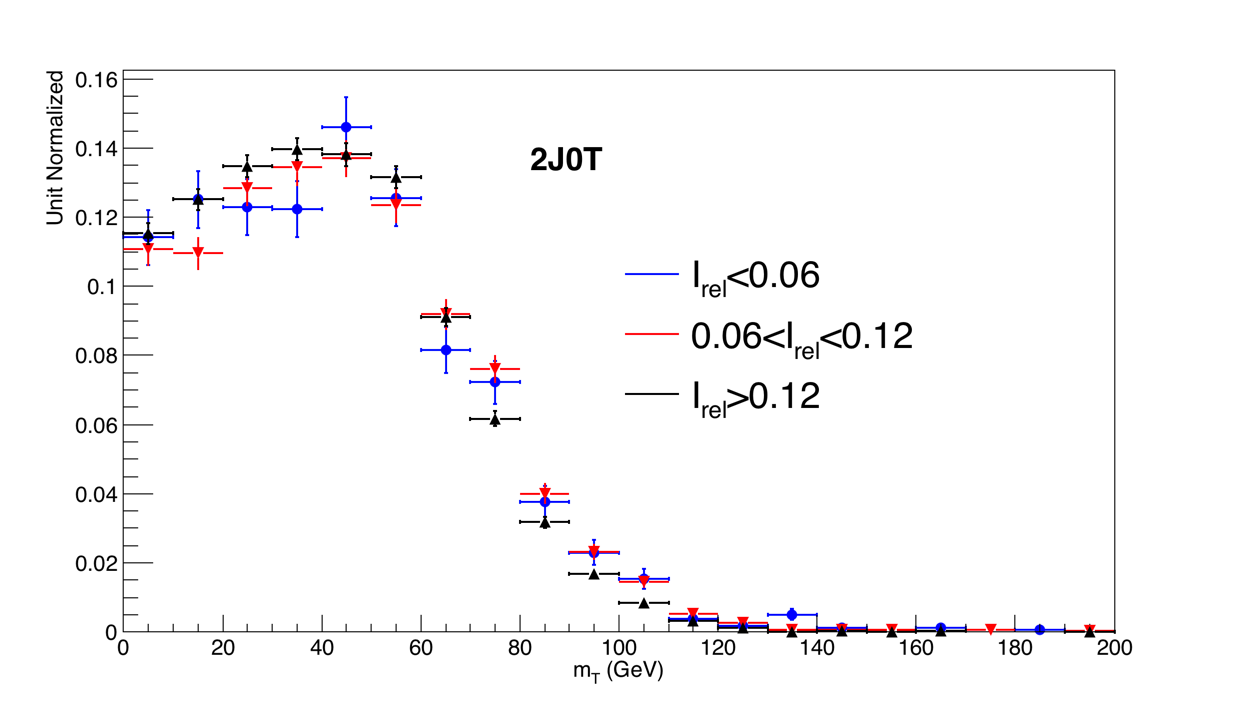
\includegraphics[width=0.45\textwidth]{figures/2J0T/Sep3/QCD_mtW_shape_Comparison.png}
\caption{\label{fig:qcdshape}Comparison of the m$_{T}$ shape for \QCD between isolated , moderately isolated  and anti-isolated region of 2J0T}
\end{center}
\end{figure}


\subsection{Estimation of the QCD-contribution in 2J0T}
\label{sec:qcd2J0T}
The transverse mass ($\mT$) of the $(\mu,\met)$ system provides good discrimination power between QCD and processes with prompt muons. An extended maximum likelihood fit with 2 parameters is performed to the $\mT$ distribution of in the 2J0T region. We assume that the \mT distribution in data F($\mT$) can be parametrized as 

\begin{center}
\begin{equation}
\label{eq:QCDFit}
F(\mT) = N_{\rm QCD} \cdot Q(\mT) + N_{\rm nonQCD} \cdot B(\mT)  ,
\end{equation}
\end{center}

where $Q(\mT)$ stands for the QCD \mT-template  taken from the anti-isolated region of 2J0T as described above, $B(\mT)$ is the non-QCD $\mT$-template obtained by summing up 
the simulated contributions from all other processes with prompt muons in the isolated region according to their predicted cross section. Both templates, $Q(\mT)$  and $B(\mT)$ are normalized to an integral of 1.0. The fit parameter $N_{\rm QCD}$ denotes the number of QCD events and $N_{\rm nonQCD}$ represents the total number of non-QCD events. The $N_{\rm QCD}$ and $N_{\rm nonQCD}$ parameters are allowed to float during the fit to the \mT distribution performed as shown in Figure~\ref{fig:qcdFit1} and ~\ref{fig:qcdFit2}.\\   
 The entire range of the \mT-distribution is fitted. From the resulting \QCD yield we extrapolate the \QCD-contribution to the signal region ($\mt > 50\,$\GeV) by calculating the integral of the \mT-distribution from \QCD normalized to the fit-result from $\mT = 50\,$\GeV to infinity.\\
 The QCD \mT-template is derived from data in the anti-isolated sideband region ($\murelIso > 0.12$), as described above, while the actual fit is performed in the signal region ($\murelIso < 0.06$). 

As a further cross check also an unbinned fit is performed. The fitted (and extrapolated) yields from the different types of fits to $\mT$ are summarized in Table~\ref{tab:QCDFitSF1}. Overall a good agreement between the different fits can be observed. A fit based on missing transverse energy instead of $\mT$ can be found in Appendix~\ref{app:METFit_2J0T}.


\begin{figure}[hbpt]
\begin{center}
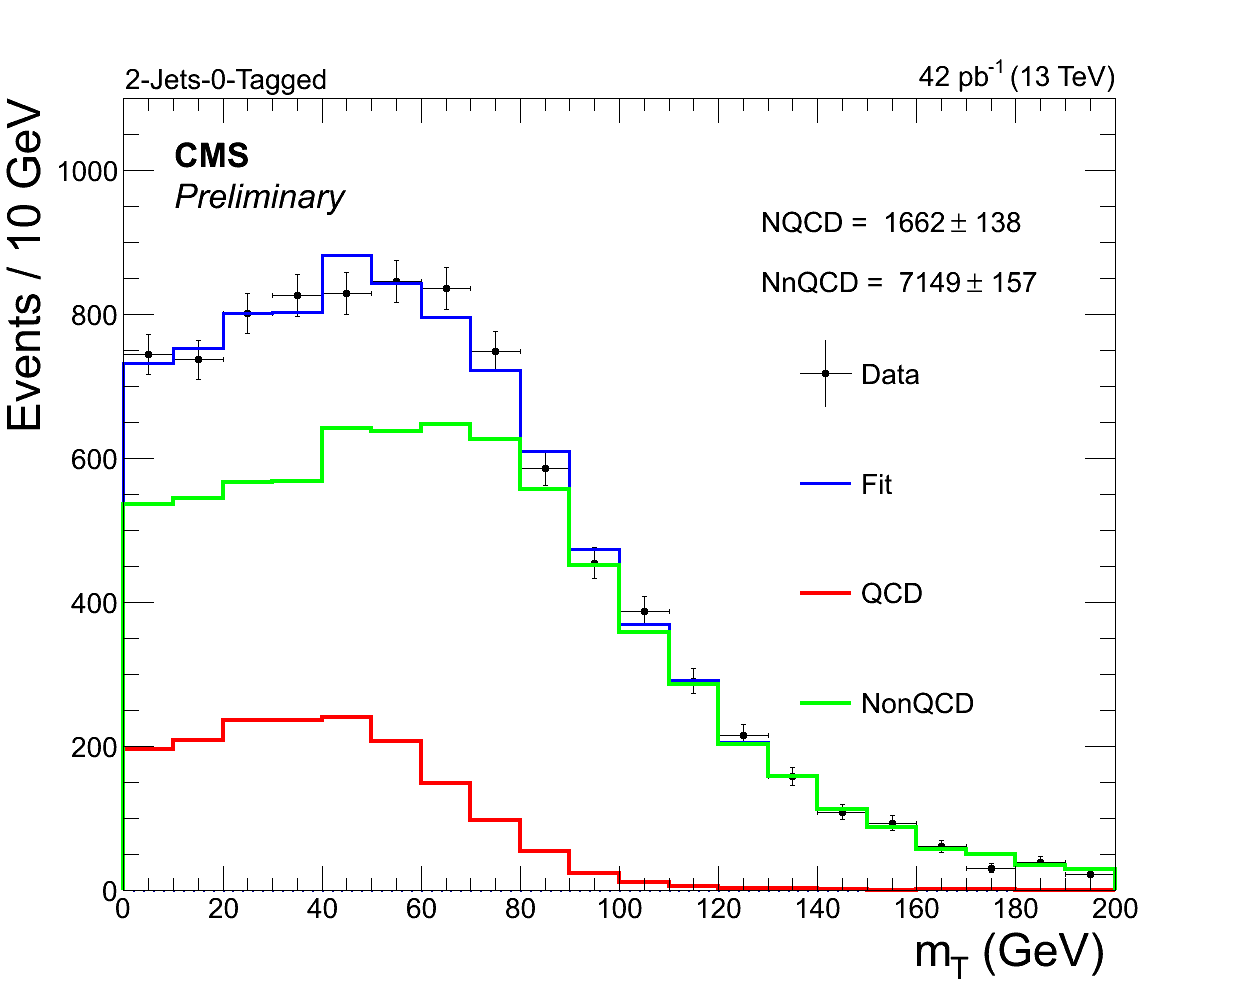
\includegraphics[width=0.45\textwidth]{figures/2J0T/Sep8/BinnedFit_QCD_MC.png}
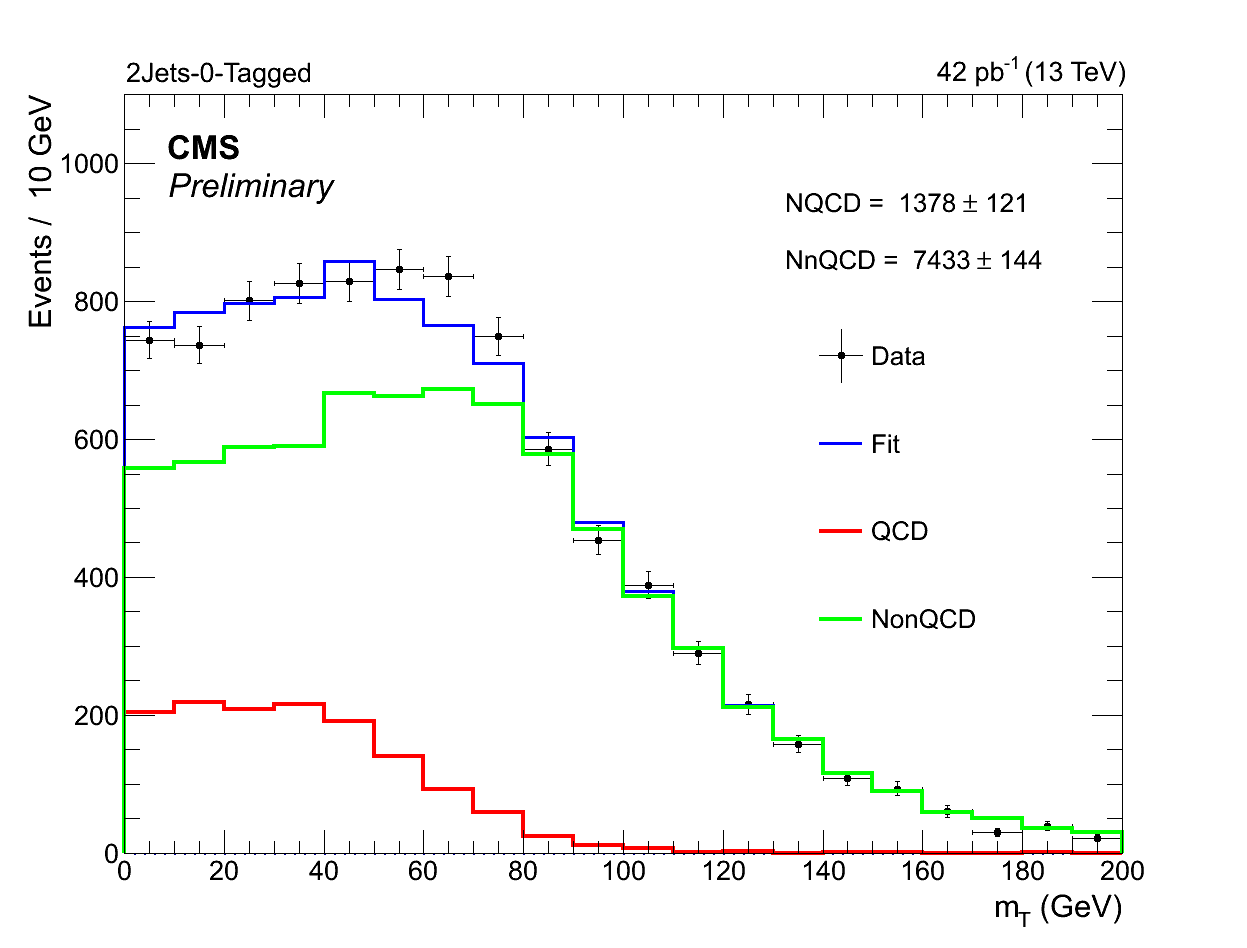
\includegraphics[width=0.45\textwidth]{figures/2J0T/Sep8/BinnedFit_QCD_DD.png}\hfill
%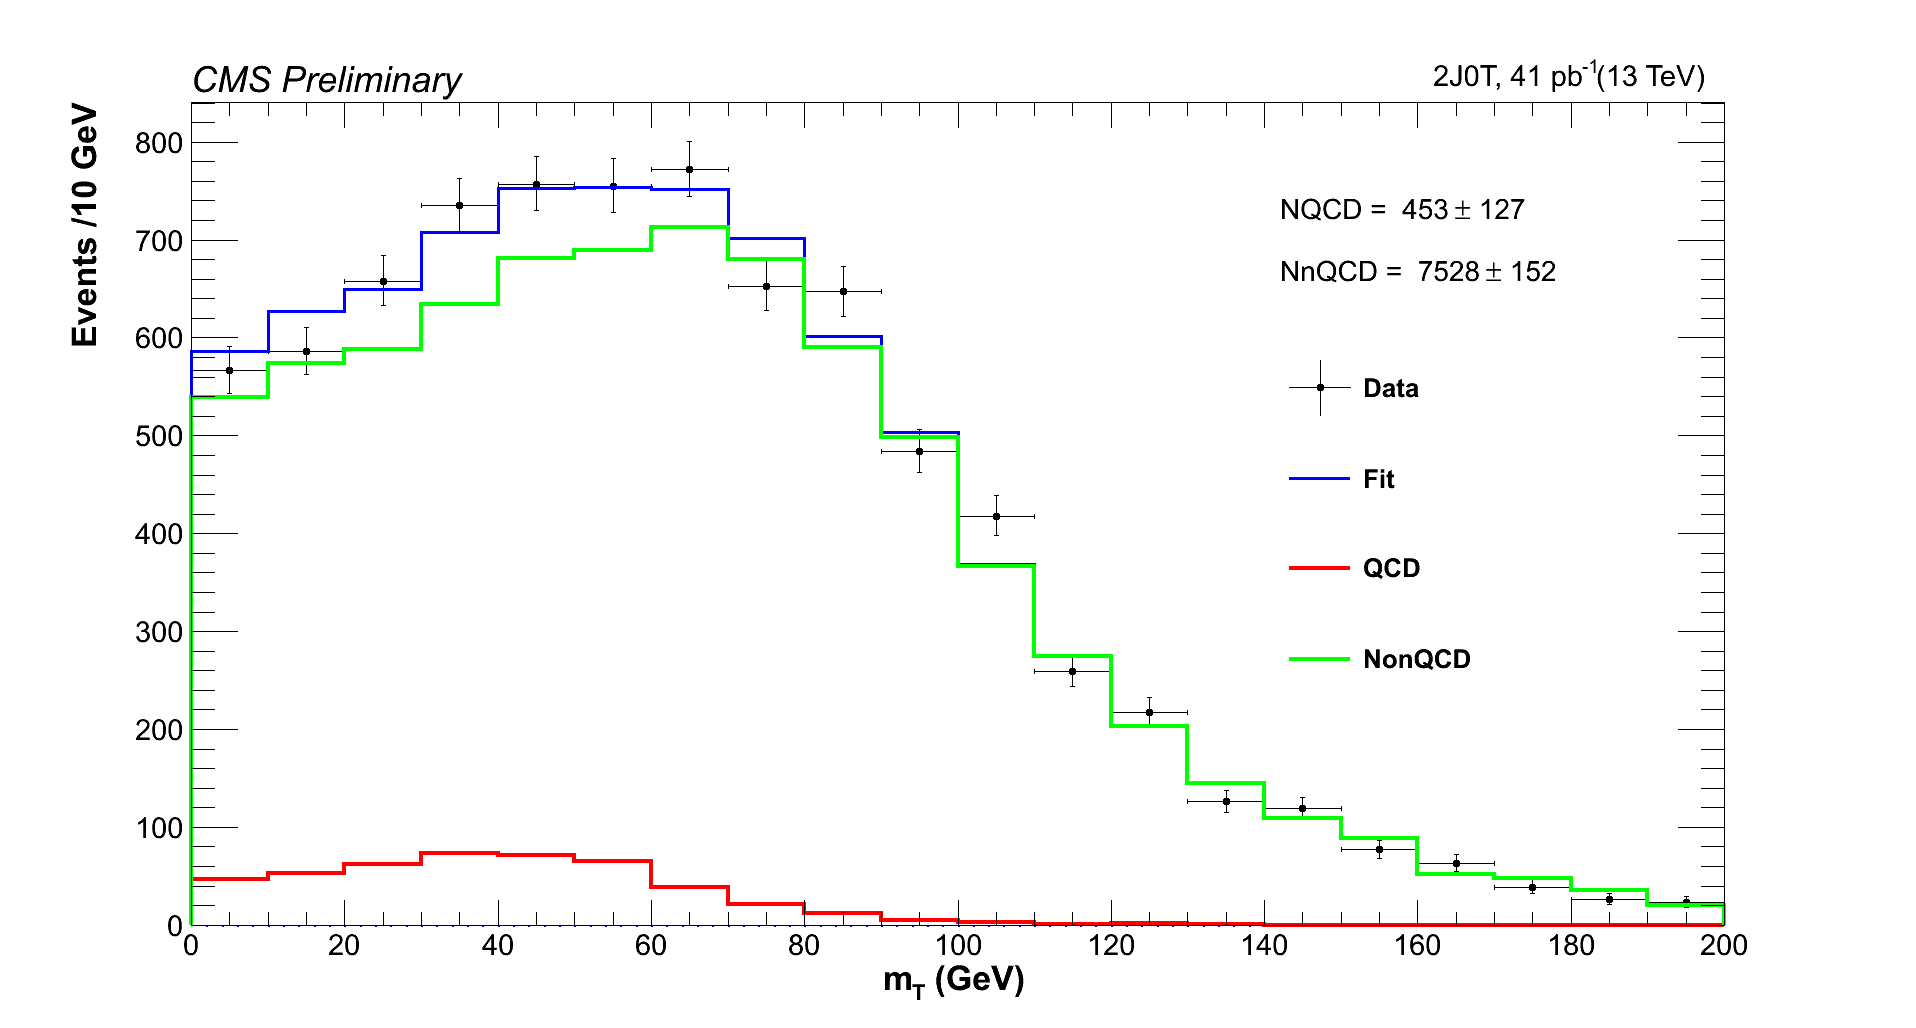
\includegraphics[width=0.45\textwidth]{figures/2J0T/Data_BinnedFit_QCD_DD.png}
\caption{\label{fig:qcdFit1}Post fit distribution of $\mT$ for binned fit where QCD shape is taken from MC (left) and data-driven (right) }
\end{center}
\end{figure}

\begin{figure}[hbpt]
\begin{center}
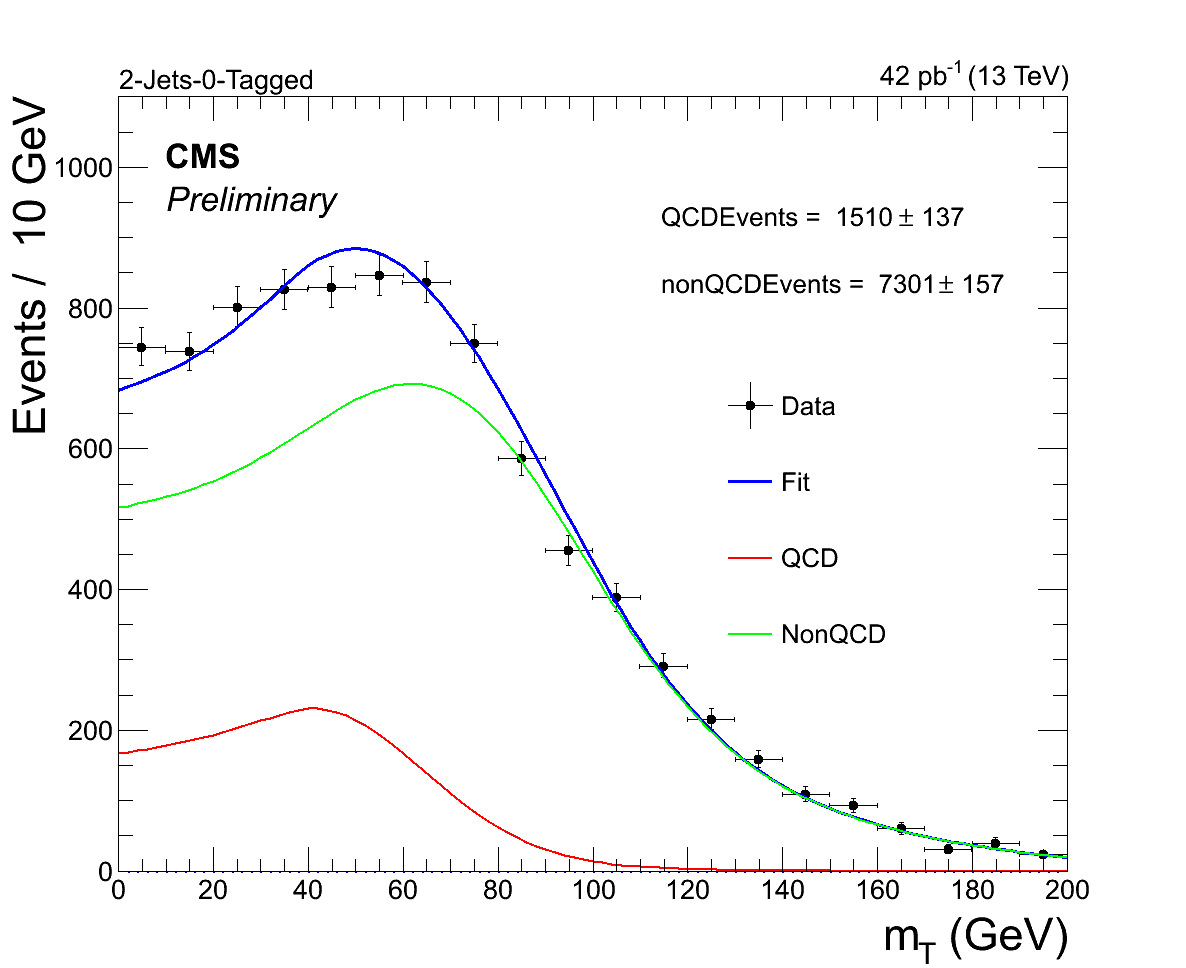
\includegraphics[width=0.6\textwidth]{figures/2J0T/Sep8/UnbinnedFit_QCD.png}
\caption{\label{fig:qcdFit2}Post fit distribution of $\mT$ for unbinned fit}
\end{center}
\end{figure}




\begin{table}
\begin{center}
\caption{QCD estimation in the 2J0T region}
\label{tab:QCDFitSF1}
\begin{tabular}{|c|c|c|c|c|c|}
\hline
Variable & Fit Type & QCD shape & Process & Fitted Yield & Extrapolated Yield\\
 & & & & (full range) & ($\mT>50$GeV) \\
\hline 
\multirow{6}{*}{\mT} & \multirow{2}{*}{Unbinned} & \multirow{2}{*}{Parametric} & QCD & 1510$\pm$137 & 501$\pm$46 \\\cline{4-6}
 & & & nonQCD & 7301$\pm$157 & 4407$\pm$95 \\\cline{2-6}
 & \multirow{4}{*}{Binned} & \multirow{2}{*}{From MC} & QCD & 1662$\pm$138 & 547$\pm$46 \\\cline{4-6}
 & & & nonQCD & 7149$\pm$157 & 4291$\pm$94 \\\cline{3-6}																		
 & & \multirow{2}{*}{Data Driven} & QCD & 1378$\pm$121 & 342$\pm$30 \\\cline{4-6}
 & & & nonQCD & 7433$\pm$144 & 4462$\pm$86 \\\cline{3-6}						   
\hline 
%\multirow{4}{*}{\met} & \multirow{4}{*}{Binned}& \multirow{2}{*}{From MC} & QCD & 2216$\pm$118 & 461$\pm$25 \\\cline{4-6}
% & & & nonQCD & 5804$\pm$133 & 3092$\pm$71 \\\cline{3-6}
% & & \multirow{2}{*}{Data Driven} & QCD & 1615$\pm$90 & 174$\pm$10 \\\cline{4-6}
% & & & nonQCD & 6406$\pm$114 & 3413$\pm$61 \\\cline{3-6}
%\hline
\end{tabular}
\end{center}
\end{table}




\newpage
\subsection{Modelling of the QCD background in 2J1T}
\label{sec:qcd2J1T}
The same procedure (inverting the relative isolation of the muon) is applied to the 2J1T region after the full selection inside and outside the top quark mass window used for signal extraction defined. Figure~\ref{fig:qcdShapeComparison2J1TmtW} shows a comparison of the \mT distribution between simulated QCD events in the isolated ( $\PFrelIso < 0.06$) against the anti-isolated region ($\PFrelIso > 0.12$), and in the intermediate region ($0.06 < \PFrelIso < 0.12$) against the  anti-isolated region. Good agreement in the shapes of the distributions from the different regions considered is found. 

Using samples of simulated events from all relevant signal and background processes the \QCD of the anti-isolated region seems overwhelming, as Table~\ref{tab:QCDEstimation2J1T} and Figure~\ref{fig:sampleComparisonDifferentIsoRegions2J1TmtW} indicate. 


\begin{table}[h!] \begin{center}
\caption{QCD and nonQCD expectation in 2J1T region for \mylumi~pb$^{-1}$} \label{tab:QCDEstimation2J1T} \resizebox{\textwidth}{!}{\begin{tabular}{|l|l|l|c @{$\pm$} l|c @{$\pm$} l|c @{$\pm$} l|} \hline $m_{\ell\nu\mathrm{b}}$ range & Cut & Process & \multicolumn{2}{c|}{$\PFrelIso < 0.06$}  &  \multicolumn{2}{c|}{$0.06< \PFrelIso < 0.12$} &\multicolumn{2}{c|}{$\PFrelIso > 0.12$}\\ \hline
\multirow{4}{*}{inclusive} & \multirow{2}{*}{No Cut} & QCD & 204&14 & 194&14&534&23\\\cline{3-9} & & nonQCD & 520&7 & 75&3 &42&2\\\cline{2-9} & \multirow{2}{*}{$m_{T}\  \rm{of\  W} >$ 50 GeV} & QCD & 58&8 & 50&7\\\cline{3-7} & & nonQCD &355&6 & 52&2\\\cline{2-7} \hline

\multirow{4}{*}{outside window} & \multirow{2}{*}{No Cut} & QCD & 59&8 & 55&7&153&12\\\cline{3-9} & & nonQCD & 201&5 & 25&1.5 &12&1\\\cline{2-9} & \multirow{2}{*}{$m_{T}\  \rm{of\  W} >$ 50 GeV} & QCD & 11&3 & 19&4\\\cline{3-7} & & nonQCD &130&4 & 16&1.1\\\cline{2-7} \hline

\multirow{4}{*}{inside window} & \multirow{2}{*}{No Cut} & QCD & 145&12 & 138&11&381&20\\\cline{3-9} & & nonQCD & 335&5 & 51&2 &30&1\\\cline{2-9} & \multirow{2}{*}{$m_{T}\  \rm{of\  W} >$ 50 GeV} & QCD & 47&7 & 31&5\\\cline{3-7} & & nonQCD &236&4 & 36&1.5\\\cline{2-7} \cline{1-7} 

\end{tabular}} \end{center} \end{table} 


\begin{figure}[H!]
\begin{center}
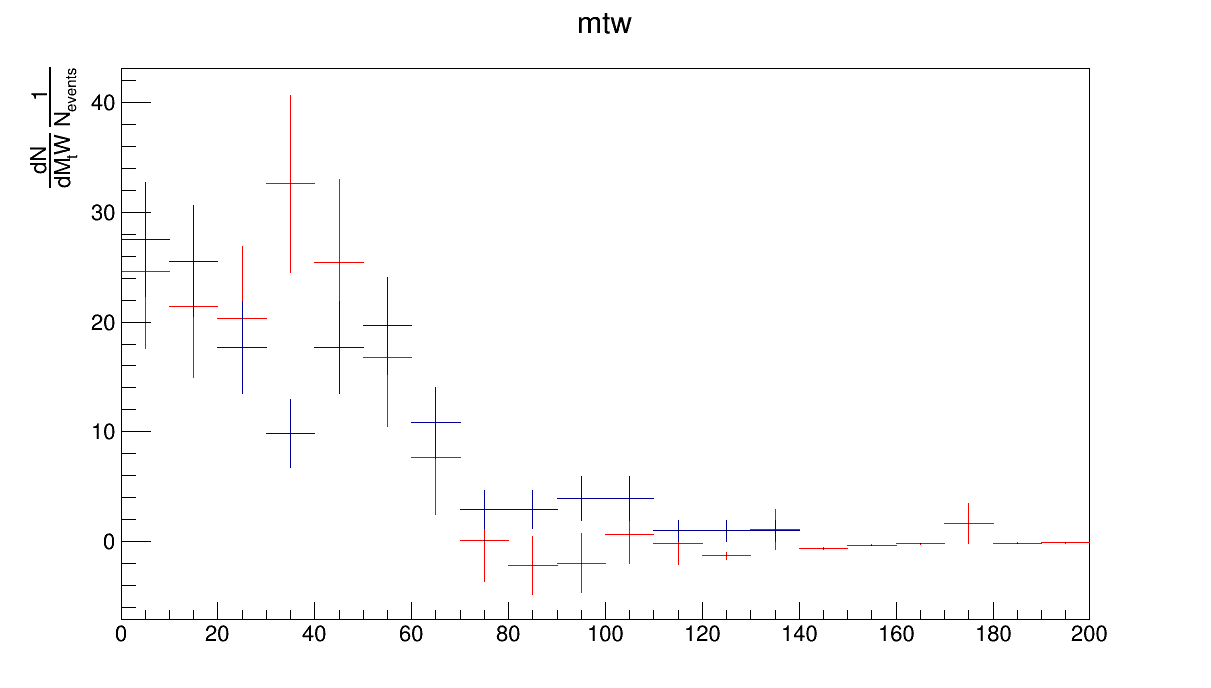
\includegraphics[width=6.5cm]{figures/2J1T/MTW_QCD_lessiso_vs_antiso_SR.png}
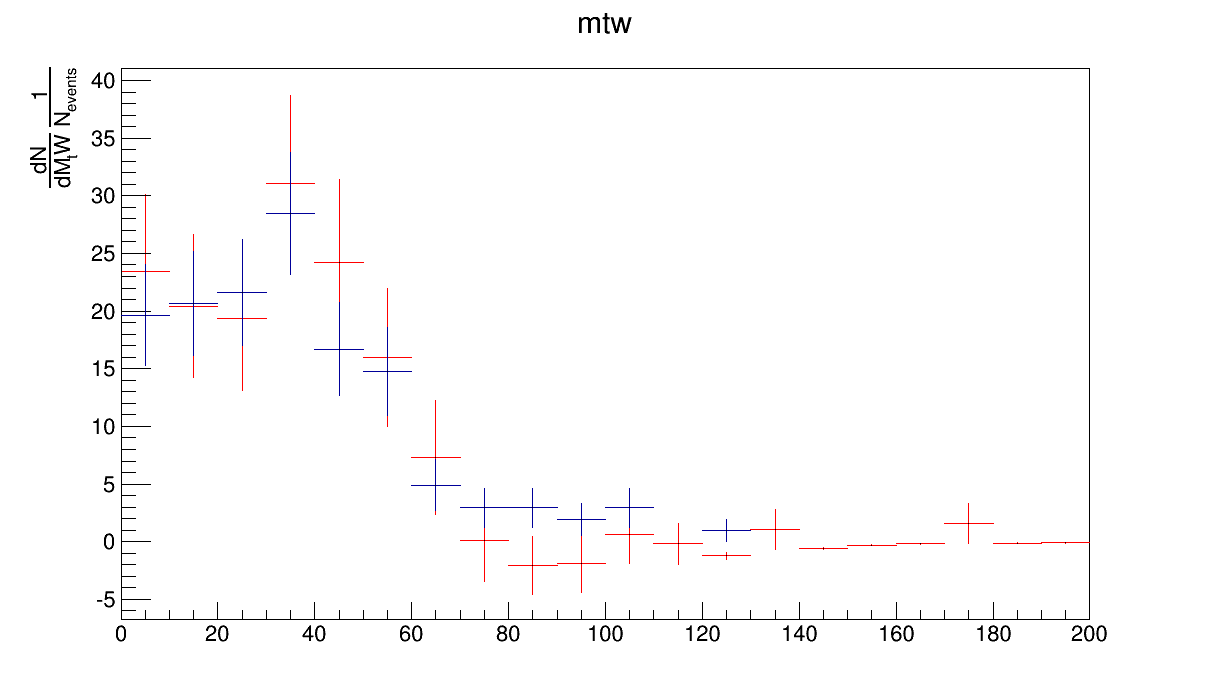
\includegraphics[width=6.5cm]{figures/2J1T/MTW_QCD_moreiso_vs_antiso_SR.png}
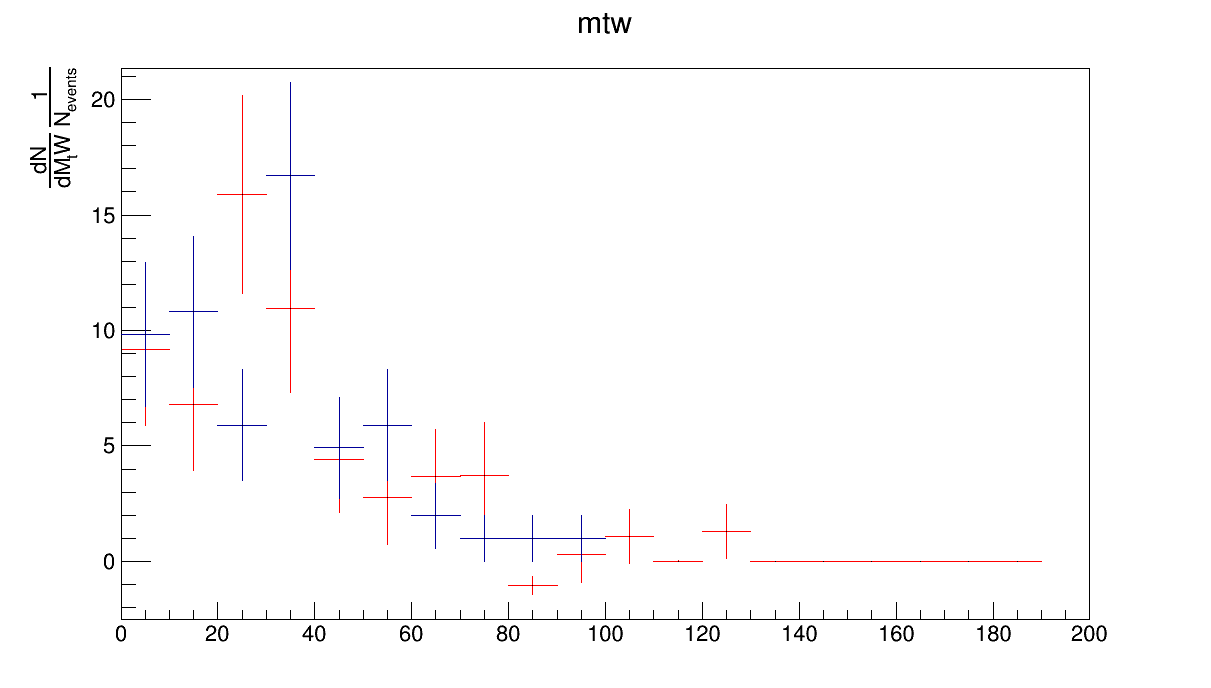
\includegraphics[width=6.5cm]{figures/2J1T/MTW_QCD_lessiso_vs_antiso_SB.png}
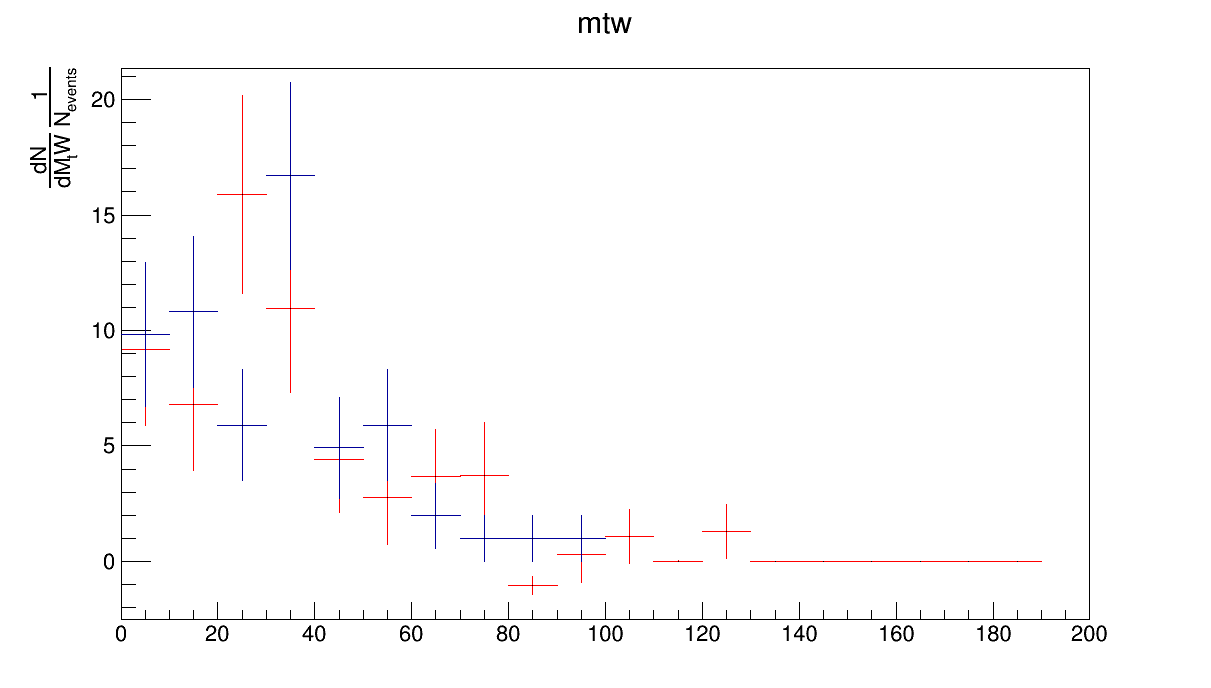
\includegraphics[width=6.5cm]{figures/2J1T/MTW_QCD_lessiso_vs_antiso_SB.png}
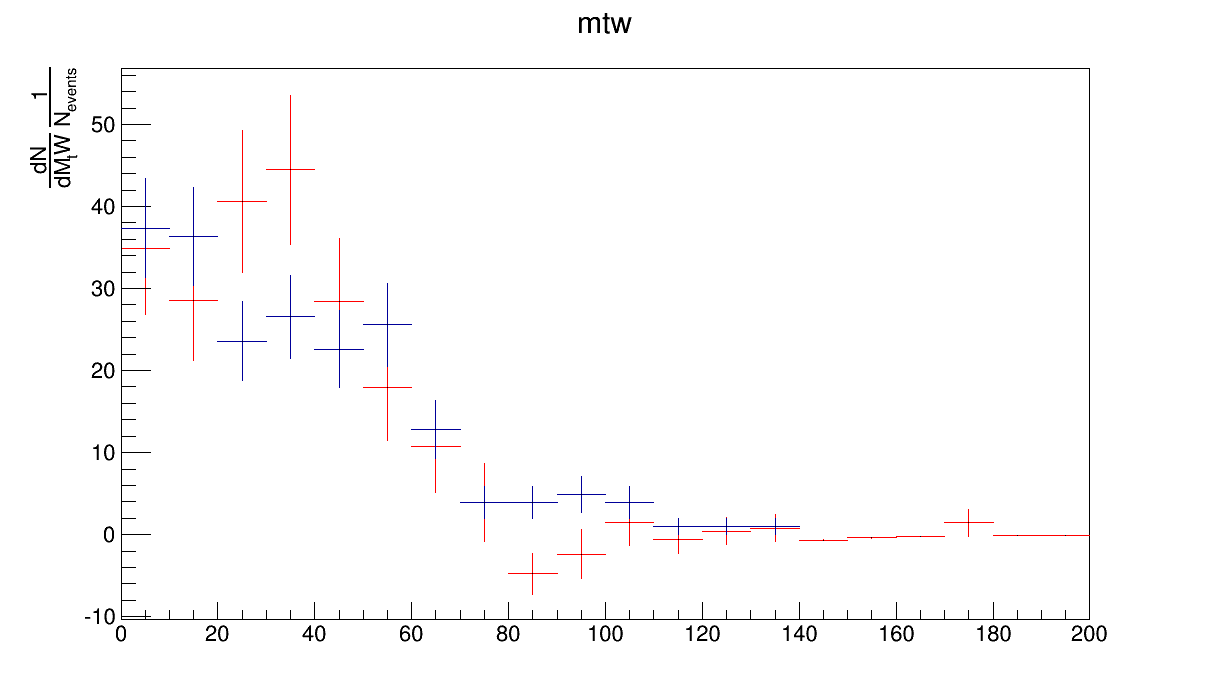
\includegraphics[width=6.5cm, height=4.4cm]{figures/2J1T/MTW_QCD_lessiso_vs_antiso_inclusive_mTop.png}
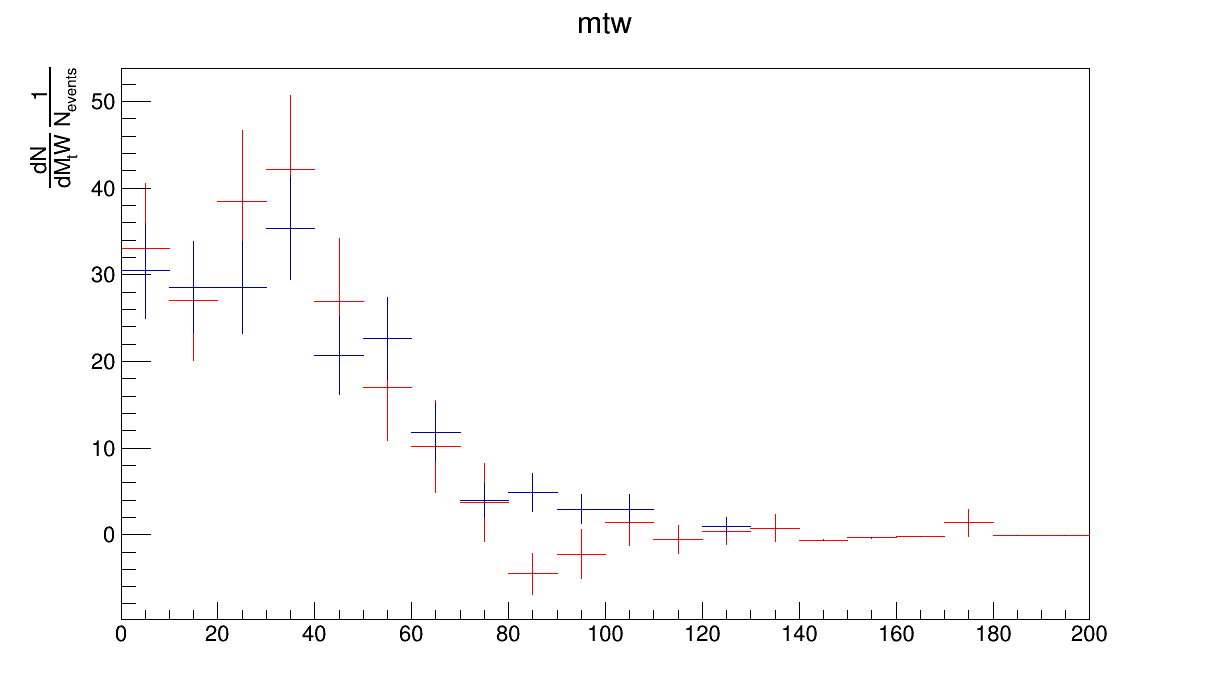
\includegraphics[width=6.5cm]{figures/2J1T/MTW_QCD_moreiso_vs_antiso_inclusive_mTop.png}\hfill
\caption{\label{fig:qcdShapeComparison2J1TmtW} Comparison of the distributions of $\mT$ from the anti-isolated region with the distribution from the isolated region (left), and with the distribution from the intermediate region (right). The distribution from the anti-isolated region is plotted with the red marker, and scaled to the integral of either the isolated or the intermediate distribution, respectively. From the top to the bottom: the SR ($130<\topMass<225\,$\GeV), the SB region and without applying any cut on $\topMass$.}
\end{center}
\end{figure}


\begin{figure}[h]
\begin{center}
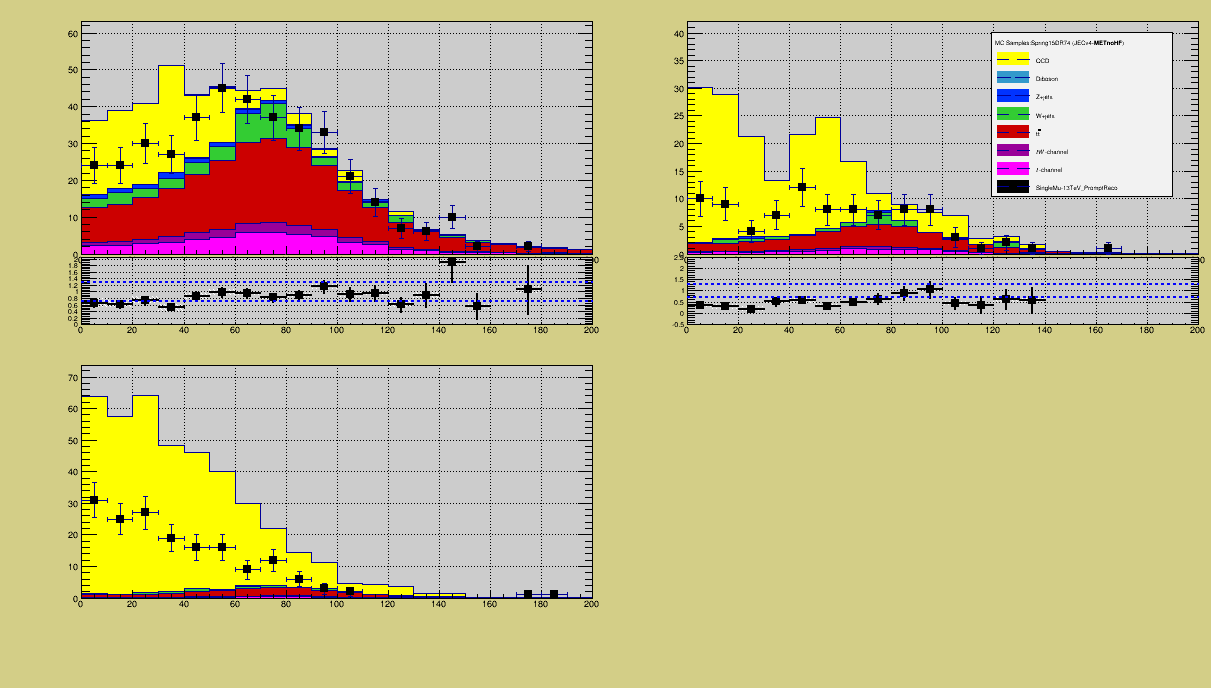
\includegraphics[width=9.5cm]{figures/2J1T/MTW_Different_iso_regions_SR.png}
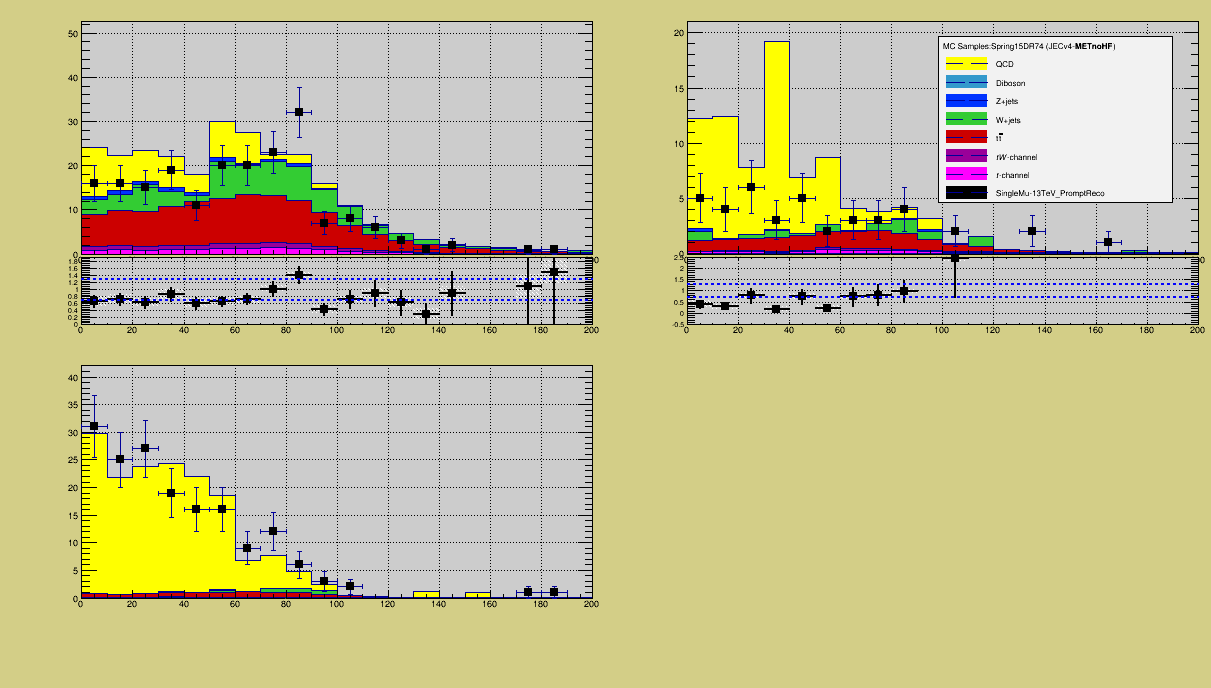
\includegraphics[width=9.5cm]{figures/2J1T/MTW_Different_iso_regions_SB.png}
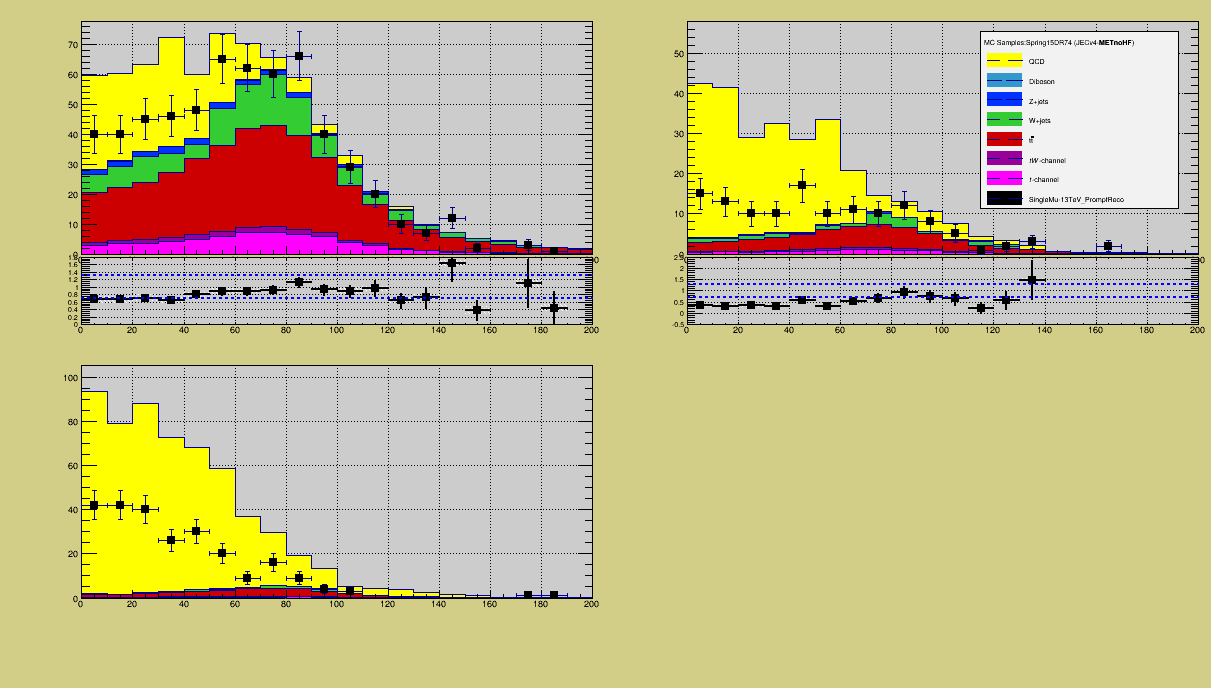
\includegraphics[width=9.5cm]{figures/2J1T/MTW_Different_iso_regions_inclusive_mTop.png}
\caption{\label{fig:sampleComparisonDifferentIsoRegions2J1TmtW} Comparison of the distributions of $\mT$ in the isolated region (upper left), in the intermediate region (upper right), and in the anti-isolated region (bottom left). From top to bottom: the SR ($130<\topMass<225\,$\GeV), the SB region and without applying any cut on $\topMass$.}
\end{center}
\end{figure}
 
 \clearpage

\subsection{Estimation of the QCD-contribution in 2J1T}

The same binned likelihood fit as in the 2J0T control region is applied to the \mT distribution in the 2J1T region. The template for the non-\QCD processes is again derived from MC simulation by summing up the individual contributions from the different processes weighted with the corresponding cross sections, while the \QCD-template is again derived from the anti-isolated sideband in data ($\murelIso > 0.12$). Again, the entire \mT-distribution is fitted and the \QCD contribution in the signal region ($\mT > 50\,$\GeV) is extrapolated from the post-fit-\mT-distribution, normalized to the fit results. Table ~\ref{tab:QCDExpectation2J1TNoSys} reports the fitted \QCD and non-\QCD yields for the three fit scenarios.

\begin{table}[b]
\begin{center}
\caption{QCD and nonQCD estimation in the isolated 2J1T region. Uncertainties are determined by the procedure in sec. ~\ref{sec:qcd2J1Txchecks}.}
\label{tab:QCDExpectation2J1TNoSys}
\begin{tabular}{|c|c|c|c|}
\hline
 $m_{\ell\nu\mathrm{b}}$ range& Process & Fitted Yield & Extrapolated Yield  \\
                              &         & (full \mT range) &   ($\mT> 50\,$\GeV) \\
\hline
 \multirow{2}{*}{inclusive} & QCD & 82$\pm$22 & 12$\pm$5 \\
 & nonQCD & 514$\pm$28 & 351$\pm$19 \\
 \hline
 \multirow{2}{*}{outside window} & QCD & 20$\pm$13 & 2$\pm$1.1 \\
         & nonQCD & 181$\pm$16 & 116$\pm$10 \\
\hline
\multirow{2}{*}{inside window} & QCD & 65$\pm$17 & 10$\pm$4.7 \\
                         & nonQCD & 330$\pm$22 & 232$\pm$15 \\
\hline
\end{tabular}
\end{center}
\end{table}




\begin{figure}[h!]
\begin{center}
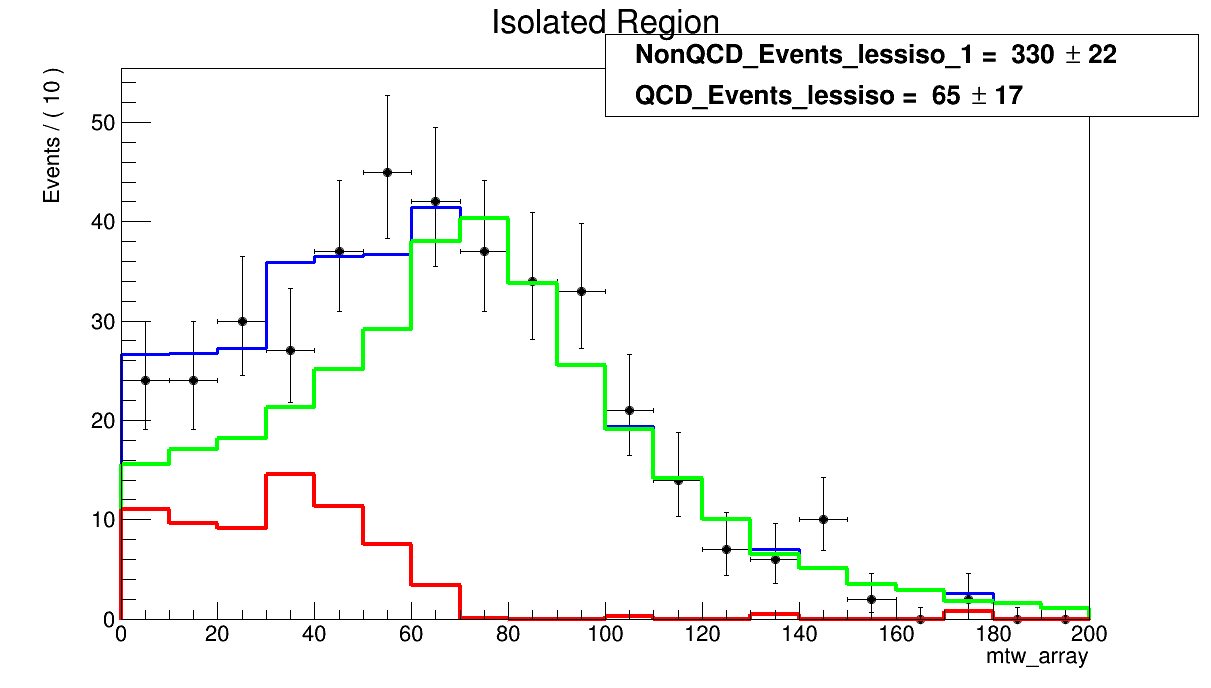
\includegraphics[width=6.5cm]{figures/2J1T/MTW_fit_2j1t_lessiso_SR.png}
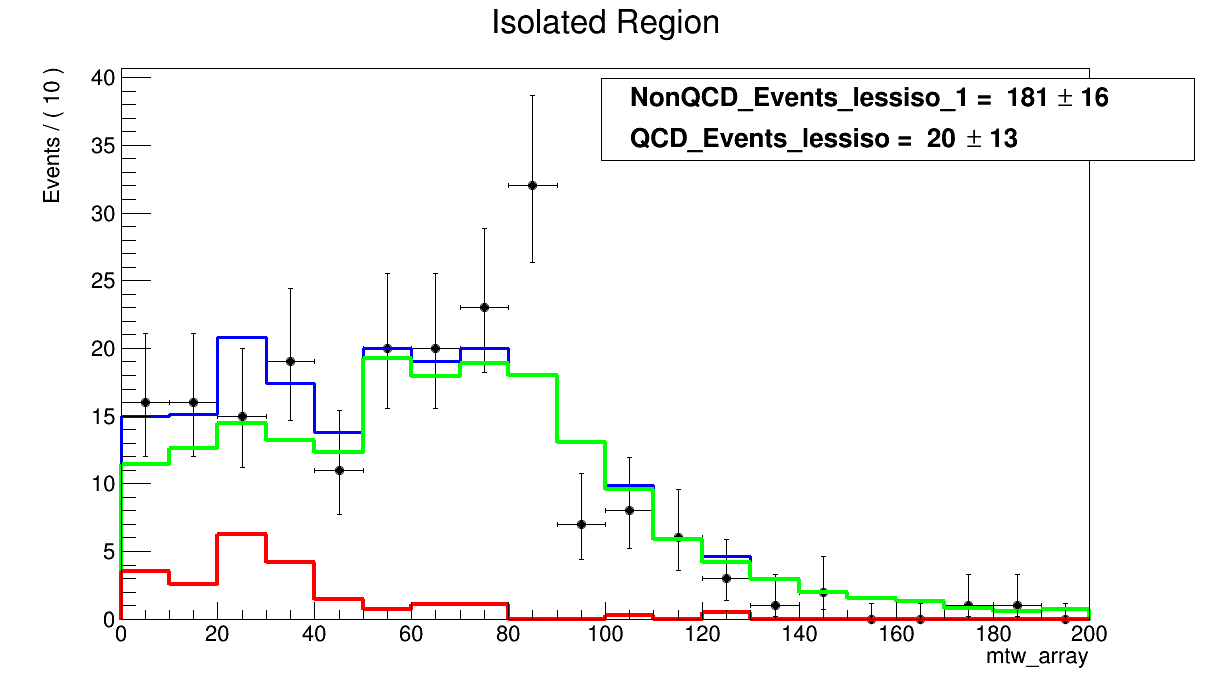
\includegraphics[width=6.5cm]{figures/2J1T/MTW_fit_2j1t_lessiso_SB.png}\hfill
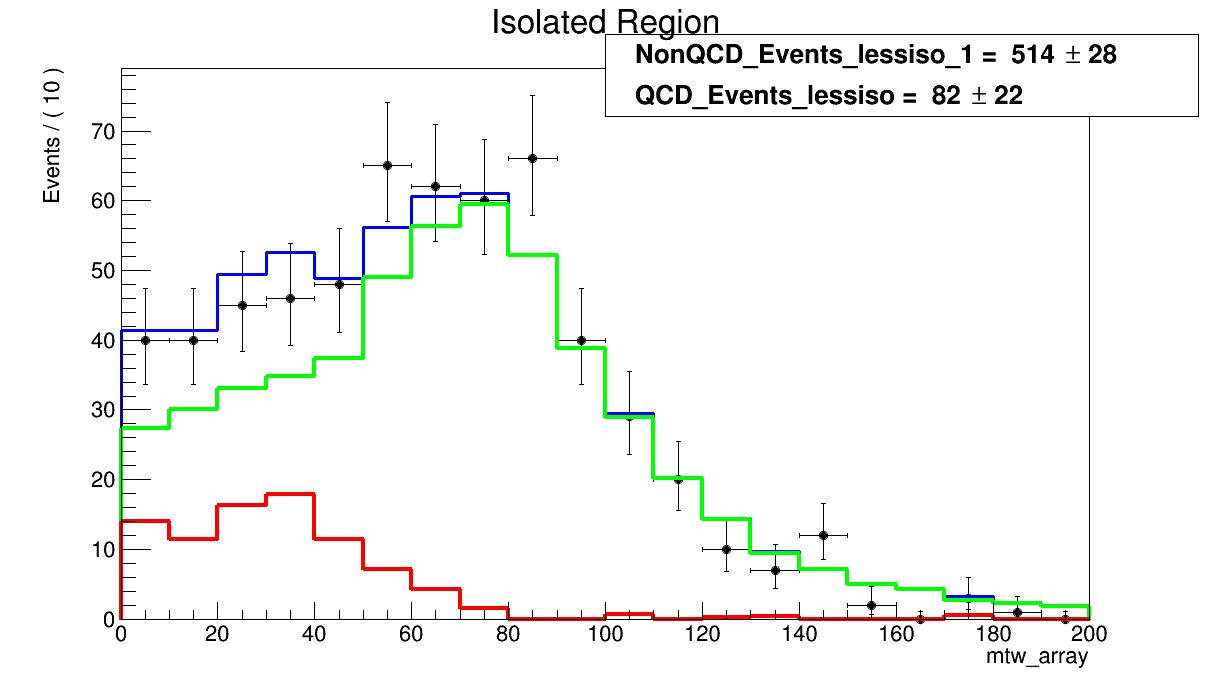
\includegraphics[width=6.5cm]{figures/2J1T/MTW_fit_2j1t_lessiso_inclusive_mTop_range.png}
\caption{\label{fig:qcdFit2J1TmtWLessIso} Fit in the isolated region ($\PFrelIso < 0.06$): Fit results of $\mT$ inside (left) and outside (right) the $130<\topMass<225\,$\GeV window, and without applying any cut (``inclusive'') on $\topMass$ (bottom).  }
\end{center}
\end{figure}

\begin{figure}[h!]
\begin{center}
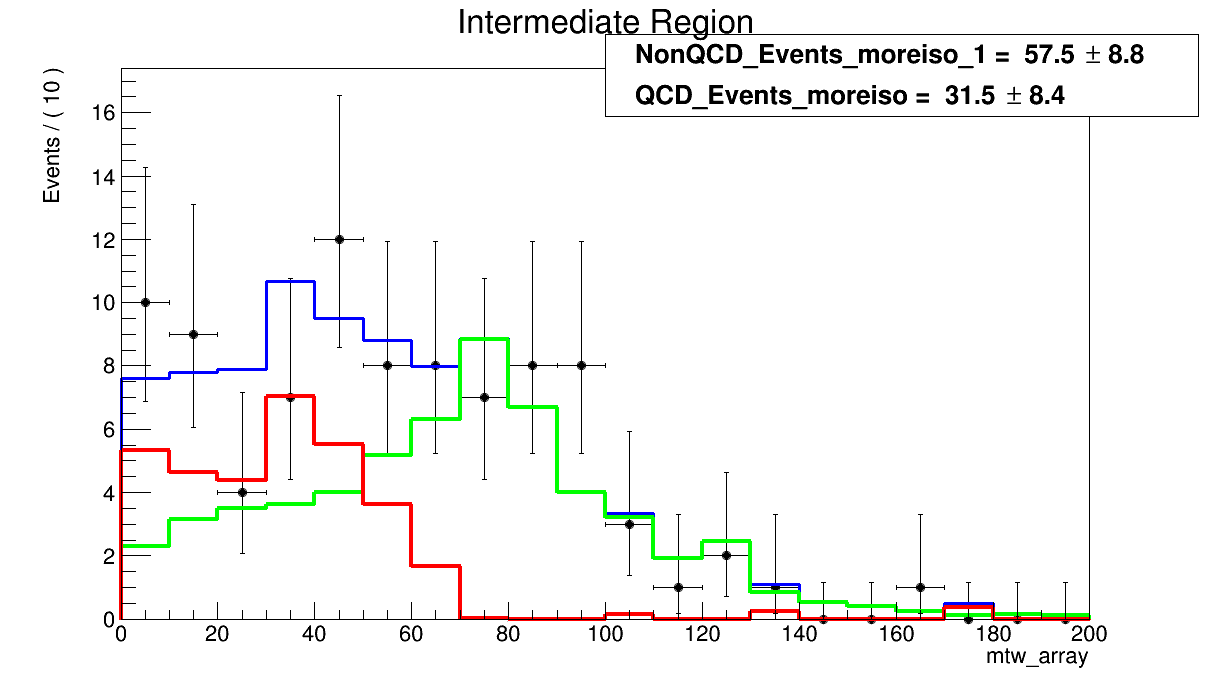
\includegraphics[width=6.5cm]{figures/2J1T/MTW_fit_2j1t_moreiso_SR.png}
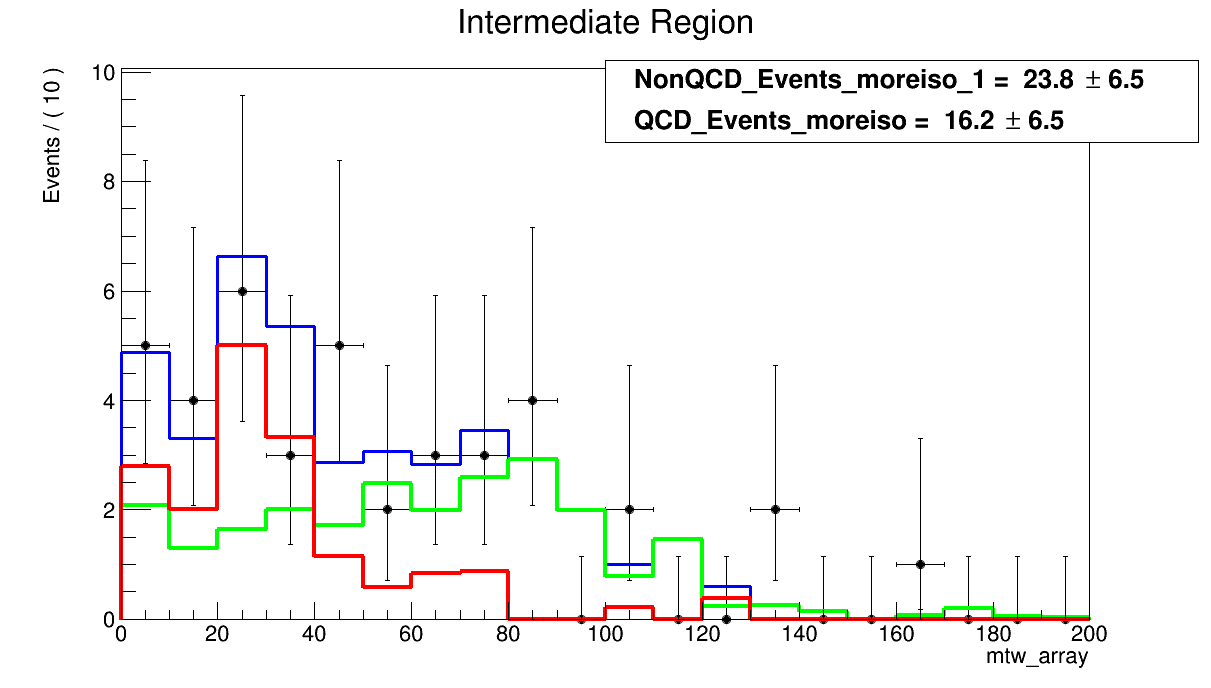
\includegraphics[width=6.5cm]{figures/2J1T/MTW_fit_2j1t_moreiso_SB.png}\hfill
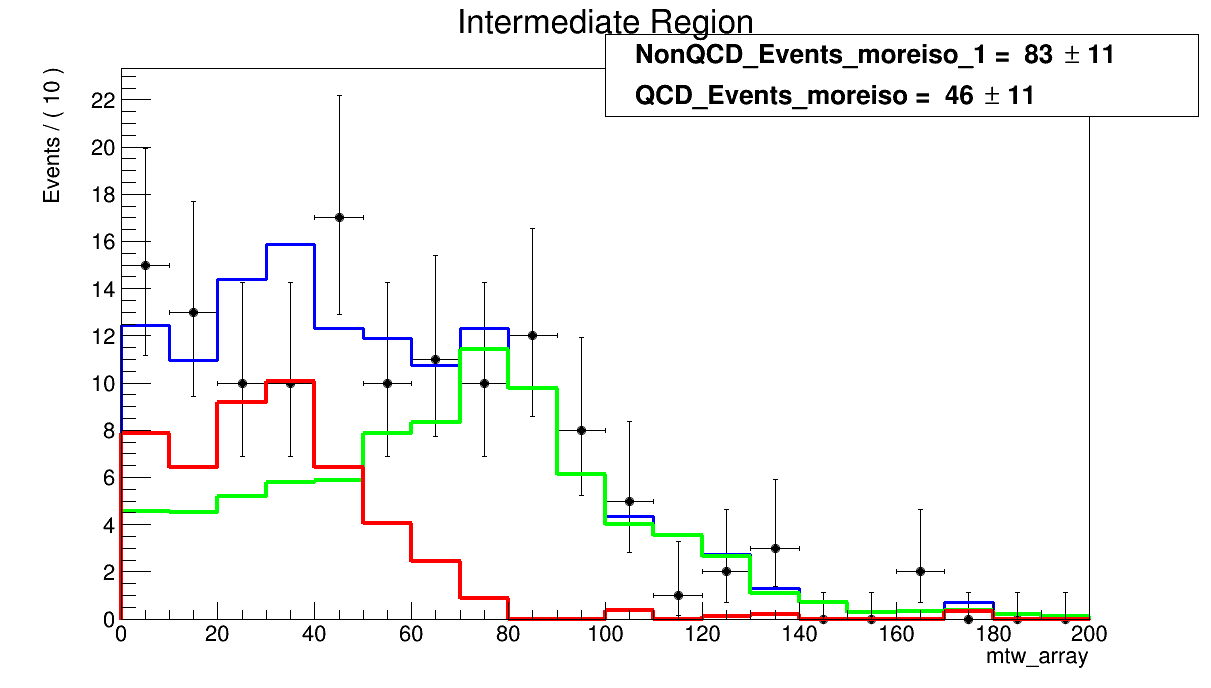
\includegraphics[width=6.5cm]{figures/2J1T/MTW_fit_2j1t_moreiso_inclusive_mTop_range.png}
\caption{\label{fig:qcdFit2J1TmtWMoreIso} Fit in the intermediate region ($0.06< \PFrelIso < 0.12$): Fit results of $\mT$ inside (left) and outside (right) the $130<\topMass<225\,$\GeV window, and without applying any cut (``inclusive'') on $\topMass$ (bottom). }
\end{center}
\end{figure}



Figure  ~\ref{fig:qcdFit2J1TmtWLessIso} and  ~\ref{fig:qcdFit2J1TmtWMoreIso} exhibit two represetative examples of the fitting process in the isolated region ($\PFrelIso < 0.06$) and in the intermediate region ($0.06 < \PFrelIso < 0.12$), respectively. Figure ~\ref{fig:sampleComparisonDifferentIsoRegions2J1TmtWPostFit} shows the post-fit distribution of $\mT$ inside, outside the $130<\topMass<225\,$\GeV window and in the full range.





\begin{figure}[h!]
\begin{center}
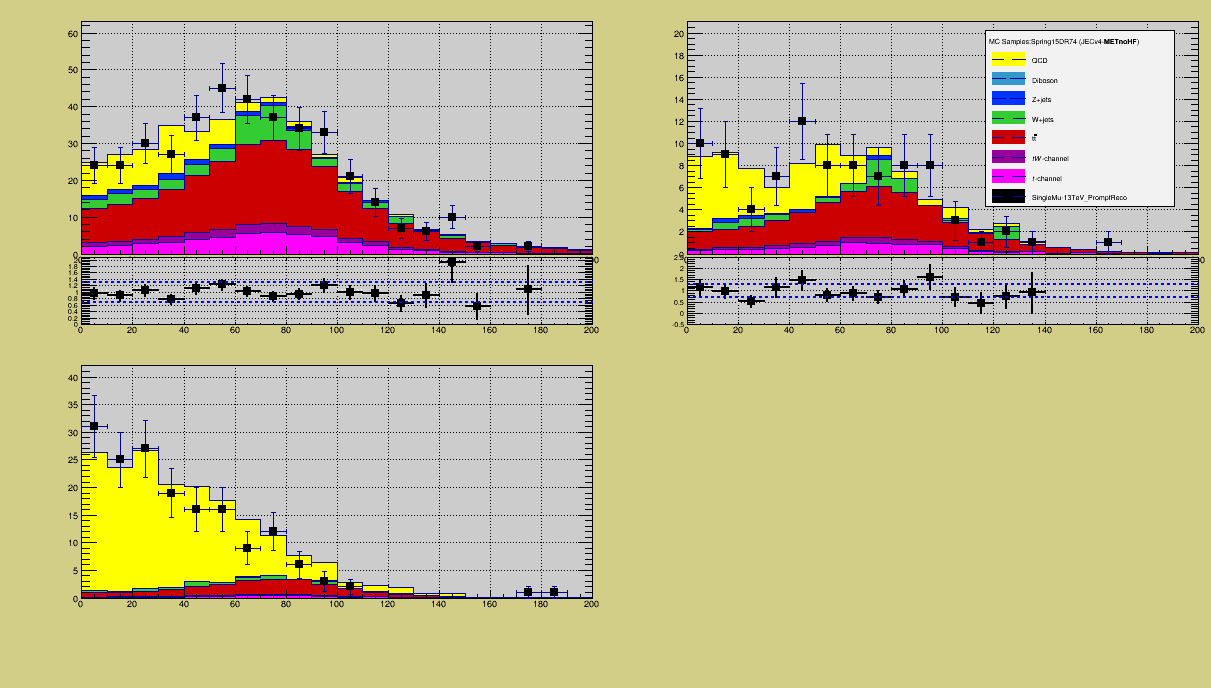
\includegraphics[width=9.5cm]{figures/2J1T/MTW_Different_iso_regions_SR_postfit.png}
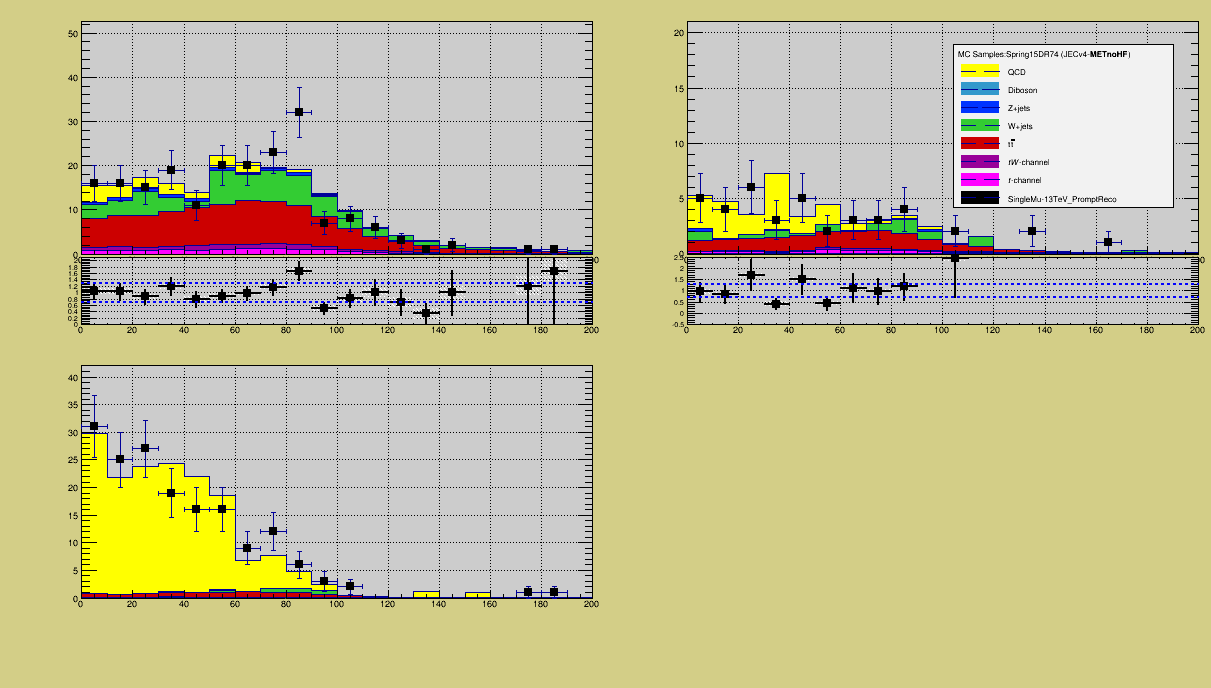
\includegraphics[width=9.5cm]{figures/2J1T/MTW_Different_iso_regions_SB_postfit.png}
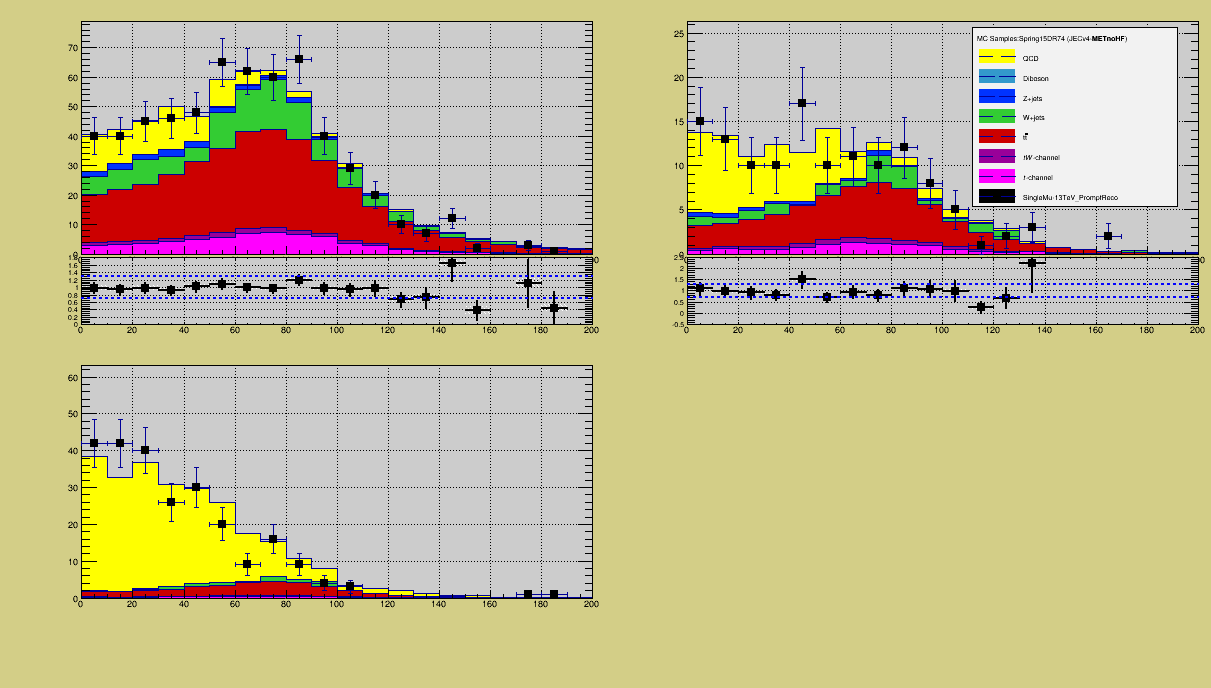
\includegraphics[width=9.5cm]{figures/2J1T/MTW_Different_iso_regions_inclusive_mTop_postfit.png}
\caption{\label{fig:sampleComparisonDifferentIsoRegions2J1TmtWPostFit}  Post fit distributions of $\mT$ in the isolated region (left) and in the intermediate region (right). From the top to the bottom: the SR ($130<\topMass<225\,$\GeV), the SB region and  without applying any cut on $\topMass$.}
\end{center}
\end{figure}

\clearpage

\subsubsection{Cross-checks}
\label{sec:qcd2J1Txchecks}
The stability of the results in Table ~\ref{tab:QCDExpectation2J1TNoSys} is tested by performing alternative fits with different settings. In addition, the cross-checked have been performed also for the intermediate ($0.06 < \PFrelIso < 0.12$) region. Plots for the cross checks summarized below can be found in Appendix~\ref{app:qcdcrosschecks}.

\subsubsection{Effect of nonQCD MC subtraction}
As the final shape is obtained by subtracting simulated non-QCD process templates from the anti-isolated data template, the resulting shape might be prone to fluctuations in the templates. To check, we variated the MC templates to be subtracted up and down. All the templates were
varied together, with uncertainties of 30$\%$ for W+jets and 20$\%$ for all the other processes. No subtraction from the anti-isolated data template has been also tried.

\subsubsection{Fit in a $\mT$ sub-range}
The fitting procedure explained above is repeated here having selected $>10 \GeV$ as the lower value of the $\mT$ variable instead of $0 \GeV$.  

\subsubsection{Fit with more nonQCD components}
The shapes of the non-QCD components might differ to some degree. To estimate the effect of this, the QCD estimation was performed by fitting 3 components instead of 2. The components were QCD, Electroweak V production (Drell-Yan and W+Jets) and top processes. 

\subsubsection{Fit with the MC template}
The effect of the shapes of the QCD component has been also examined by considering the MC template in the respective isolation region.

\subsubsection{Fit using $\met$ template}
The effect of the shapes of the non-QCD and QCD components has been also examined by considering the  $\met$ template in the respective isolation region. Fit has been performed for values greater than $>10 \GeV$ due to a slight mis-modeling of the $\met$ in the first bin.

\subsubsection{Fit using the isolated region ($\PFrelIso < 0.12$) }
In order to better constrain the uncertainty on the QCD yield, the (nomimal) fit has been performed for the isolated region ($\PFrelIso < 0.12$) and extrapolated to the isolated region ($\PFrelIso < 0.06$) based on the MC acceptance (Table ~\ref{tab:QCDEstimation2J1T}). In addition, for the isolated region ($\PFrelIso < 0.06$) the (nomimal) fit result from the intermediate-isolated region ($0.06 <\PFrelIso < 0.12$) has been  extrapolated to the isolated region ($\PFrelIso < 0.06$) based again on the MC acceptance (Table ~\ref{tab:QCDEstimation2J1T}).

%%%\subsubsection{Variation of anti-isolated region boundaries}
%%%To be added in the very next iteration.

Tables ~\ref{tab:Systematic_cross_check_QCD_yield_LessIso} and  ~\ref{tab:Systematic_cross_check_QCD_yield_MoreIso} summarise the absolute yield differences between the attempted variations, along with their accompanying uncertainties,  relative to the nominal configuration for the  $\mT>50$ ($\met>45$) case. Note that for the nominal configuration the uncertainties are only shown in the first row. In general, no significant discrepancies were found; all the differences between the attempted variations relative to the nominal configuration were less than 2$\sigma_{\rm{diff}}$ apart from each other, where $\sigma_{\rm{diff}}=\sqrt{| \sigma_{\rm{var}}^{2} - \sigma_{\rm{nom}}^{2} | }$. The final uncertainty has been taken as the absolute difference between the extrapolated result, from the $\PFrelIso < 0.12$ isolated region to the $\PFrelIso < 0.06$ isolated region, minus the nominal result. In case where this difference is less than the fitting uncertainty, it is the latter taken as the final uncertainty. Overall, an uncertainty of order 50$\%$ is revealed for all mass windows in the $\PFrelIso < 0.06$ isolated region.

\clearpage
\begin{table}[h!]

\caption{\scriptsize{isolated region ($\PFrelIso < 0.06$): Summary of cross-checks for systematic deviations on QCD yield for inclusive $\rm{m_{top}}$, SR and SB regions}} \label{tab:Systematic_cross_check_QCD_yield_LessIso} \centering %


\begin{tabular}{llccc} \hline\hline
	&	 & 	&\\ %
\multicolumn{2}{c}{Systematic \textit{Cross-Check}} & inclusive $\rm{m_{top}}$ & SR ($130<\rm{m_{top}}<225$ ) & SB \\
	&	 & 	&\\\hline %

\scriptsize{$|$nominal-variation($\pm$)$|$}   \\\hline

\scriptsize{nonQCD MC subtraction} & \scriptsize{Scaled Up} & \scriptsize{$|$12(3)-8(2)$|$} & \scriptsize{$|$10(2.4)-7(1.64)$|$} & \scriptsize{$|$2(1.2)-1.8(0.9)$|$} \\\cline{2-5} 
& \scriptsize{Scaled Down} & \scriptsize{$|$12-13(4)$|$} & \scriptsize{$|$10-12(3.3)$|$} & \scriptsize{$|$2-2.7(1.9)$|$} \\\cline{2-5} 
& \scriptsize{non subtracted} & \scriptsize{$|$12-22(8)$|$} & \scriptsize{$|$10-21(7)$|$} & \scriptsize{$|$2-3(3.5)$|$} \\\hline

\scriptsize{\mT subrange} & \scriptsize{$>10$} & \scriptsize{$|$12-11(3.2)$|$} & \scriptsize{$|$10-10.1(2.8)$|$} & \scriptsize{$|$2-2(1.3)$|$} \\\hline

\scriptsize{$\#$ nonQCD components} & \scriptsize{3} & \scriptsize{$|$12-21(6)$|$} & \scriptsize{$|$10-13(4)$|$} & \scriptsize{$|$2-8(4)$|$} \\\hline

\scriptsize{MC template} & \scriptsize{} & \scriptsize{$|$12-21(6.7)$|$} & \scriptsize{$|$10-13(4.3)$|$} & \scriptsize{$|$2-8(5.7)$|$} \\\hline

\scriptsize{$\met$ template} & \scriptsize{} & \scriptsize{$|$12-9.89(2.8)$|$} & \scriptsize{$|$10-4.1(2)$|$} & \scriptsize{$|$2-5(1.5)$|$} \\\hline

\scriptsize{$\PFrelIso$} & \scriptsize{$ < 0.12$} & \scriptsize{$|$12-9.5(1.8)$|$} & \scriptsize{$|$10-5.3(1.2)$|$} & \scriptsize{$|$2-2.5(0.6)$|$} \\\cline{2-5}

& \scriptsize{$ 0.06< \PFrelIso <0.12$} & \scriptsize{$|$12-7(1.5)$|$} & \scriptsize{$|$10-8(1.4)$|$} & \scriptsize{$|$2-1.8(0.8)$|$} \\\hline

\end{tabular} 
\end{table} 


\newline
\vspace*{2.5 cm}
\newline

\begin{table}[h!]

\caption{\scriptsize{intermediate region ($0.06 < \PFrelIso < 0.12$): Summary of cross-checks for systematic deviations on QCD yield for inclusive $\rm{m_{top}}$, SR and SB regions}} \label{tab:Systematic_cross_check_QCD_yield_MoreIso} \centering %

\begin{tabular}{llccc} \hline\hline
		&	 & 	&\\ %
	\multicolumn{2}{c}{Systematic \textit{Cross-Check}} & inclusive $\rm{m_{top}}$ & SR ($130<\rm{m_{top}}<225$ ) & SB \\
		&	 & 	&\\\hline %
	
	\scriptsize{$|$nominal-variation($\pm$)$|$}   \\\hline
	
	\scriptsize{nonQCD MC subtraction} & \scriptsize{Scaled Up} & \scriptsize{$|$6(1.5)-4.2(1)$|$} & \scriptsize{$|$5(1.1)-3(0.7)$|$} & \scriptsize{$|$1.83(0.7)-1.3(0.5)$|$} \\\cline{2-5} 
        &\scriptsize{Scaled Down} & \scriptsize{$|$6-8(2)$|$} & \scriptsize{$|$5-5.85(1.59)$|$} & \scriptsize{$|$1.83-2.39(0.98)$|$} \\\cline{2-5}
        & \scriptsize{non subtracted} & \scriptsize{$|$6-15(4)$|$} & \scriptsize{$|$5-12(3)$|$} & \scriptsize{$|$1.83-4(1.6)$|$} \\\hline
 
        \scriptsize{\mT subrange} & \scriptsize{$>10$} & \scriptsize{$|$6-5.7(1.6)$|$} & \scriptsize{$|$5-3.95(1.34)$|$} & \scriptsize{$|$1.83-1.87(0.8)$|$} \\\hline
 
        \scriptsize{$\#$ nonQCD components} & \scriptsize{$3$}& \scriptsize{$|$6-12(2.5)$|$} & \scriptsize{$|$5-10(2.46)$|$} & \scriptsize{$|$1.83-3(1.19)$|$}  \\\hline
 
        \scriptsize{MC template} & \scriptsize{} & \scriptsize{$|$6-15(4)$|$} & \scriptsize{$|$5-10(2.46)$|$} & \scriptsize{$|$1.83-2(1.2)$|$} \\\hline

        \scriptsize{$\met$ template} & \scriptsize{} & \scriptsize{$|$6-5.32(1.27)$|$} & \scriptsize{$|$5-3(1)$|$} & \scriptsize{$|$1.83-2.4(0.8)$|$} \\\hline

        \scriptsize{$\PFrelIso$} & \scriptsize{$<0.12$} & \scriptsize{$|$6-8.35(1.6)$|$} & \scriptsize{$|$5-7.34(1.4)$|$} & \scriptsize{$|$1.83-2.17(0.6)$|$} \\\hline
\end{tabular} 
\end{table} 

\clearpage

%
%The event yield of multijet QCD events in the ``2jet 1tag'' and ``2jet 0tag'' categories is measured performing a fit to the distributions of the 
%transverse mass \mTW reconstructed from the lepton and the missing energy in the muon channel, 
%and of the missing transverse energy \met itself in the electron channel.
%
%Although the \met has lower discriminating power with respect to \mtw it's not dependent from the lepton-met angular 
%correlations and is overall more robust in the electron channel.
%
%A maximum likelihood fit to the full distribution of the \mTW(\met) is 
%performed assuming that the data can be parametrized as: $F(x)= a\cdot S(x)+b\cdot B(x)$, where $x$ is the \mTW for the muon channel 
%and \met for the electron channel, $S(x)$ and $B(x)$ are the expected distributions for the sum of all processes including a W boson in the final state and 
%QCD events, respectively. $S(x)$ is taken from simulation, while $B(x)$ is extracted directly from collisions data.
%
%The QCD distributions $B(x)$ are obtained from a QCD-enriched region defined in the following way:
%\begin{itemize}
%\item \textbf{Muons:} the tight muon is required to have an isolation $I^{dBeta corr.}_{\mathrm{rel}}  >$ 0.12. 
%\item \textbf{Electrons:} the tight electron is required to have an isolation $I^{\rho corr.}_{\mathrm{rel}}  >$ 0.1. 
%\end{itemize} 
%
% Figure~\ref{fig:qcd_stability_vs_iso} shows the \mTW distribution in the 2-jets 0-tags for muons and the \met distribution in the 1-jet region for electrons, comparing the isolated and anti-isolated regions, and also several isolation scenarios.
%
%\begin{figure}[!h]
%\begin{center}
%\subfigure[]{
%%\includegraphics[angle=0,width=0.48\textwidth]{figures/MUMTW.png}}
%%\subfigure[]{
%%\includegraphics[angle=0,width=0.48\textwidth]{figures/ETEle.png}}
%%\subfigure[]{
%\includegraphics[angle=0,width=0.48\textwidth]{figures/MTWMu.png}}
%\subfigure[]{
%\includegraphics[angle=0,width=0.48\textwidth]{figures/METQCD.png}}
%\end{center}%
%\caption{\label{fig:qcd_stability_vs_iso} The $\mTW$ (a) and $\met$ (b) distribution for QCD MC events in the 2-jets 0-tags region for muons (a) and electrons (b).}
%\end{figure}
%
%
%\begin{figure}[!h]
%\begin{center}
%	    \subfigure[]{
%\includegraphics[angle=0,width=0.48\textwidth]{figures/testFitMTWDataQCDAntiIsoWSample_Mu.pdf}}
%	    \subfigure[]{
%\includegraphics[angle=0,width=0.48\textwidth]{figures/testFitMTWDataQCDAntiIsoWSample_Ele.pdf}}\\
%	    \subfigure[]{
%\includegraphics[angle=0,width=0.48\textwidth]{figures/testFitMTWDataQCDAntiIso_Mu.pdf}}
%	    \subfigure[]{
%\includegraphics[angle=0,width=0.48\textwidth]{figures/testFitMTWDataQCDAntiIso_Ele.pdf}}\\
%\end{center}%
%\caption{\label{fig:QCDFits} Fit to the $\mTW$/\met distribution in the following regions: 2-jets 0-tags (a,b), 2-jets 1-tag inclusive (c,d). The QCD model is taken from data.}
%\end{figure}
%
%\begin{figure}[!h]
%\begin{center}
%	    \subfigure[]{
%\includegraphics[angle=0,width=0.48\textwidth]{figures/testFitMTWDataQCDAntiIsoSR1_Mu.pdf}}
%	    \subfigure[]{
%\includegraphics[angle=0,width=0.48\textwidth]{figures/testFitMTWDataQCDAntiIsoSR1_Ele.pdf}}\\
%	    \subfigure[]{
%\includegraphics[angle=0,width=0.48\textwidth]{figures/testFitMTWDataQCDAntiIsoSR2_Mu.pdf}}
%	    \subfigure[]{
%\includegraphics[angle=0,width=0.48\textwidth]{figures/testFitMTWDataQCDAntiIsoSR2_Ele.pdf}}\\
%\end{center}%
%\caption{\label{fig:QCDFits_2} Fit to the $\mTW$/\met distribution in the following regions: 2-jets 1-tag SB (a,b), 2-jets 1-tag SR (c,d). The QCD model is taken from data.}
%\end{figure}
%
%The results of the fits are shown in Figg.~\ref{fig:QCDFits},~\ref{fig:QCDFits_2} for the 2-jets 0-tags and 2-jets 1-tag samples, the latter further separated in SR and SB regions (see Section~\ref{sec:selection}). %Figure ~\ref{fig:QCDFits_3} shows the results of the fit with an extra cut on the jet pt $>60 \GeVcc$ used in the inclusive cross section measurement cross .
%
%\begin{figure}[!h]
%\begin{center}
%	    \subfigure[]{
%\includegraphics[angle=0,width=0.48\textwidth]{figures/testFitPtCutMTWDataQCDAntiIso_Mu.pdf}}
%	    \subfigure[]{
%\includegraphics[angle=0,width=0.48\textwidth]{figures/testFitPtCutMTWDataQCDAntiIso_Ele.pdf}}\\
%	    \subfigure[]{
%\includegraphics[angle=0,width=0.48\textwidth]{figures/testFitPtCutMTWDataQCDAntiIsoSR1_Mu.pdf}}
%	    \subfigure[]{
%\includegraphics[angle=0,width=0.48\textwidth]{figures/testFitPtCutMTWDataQCDAntiIsoSR1_Ele.pdf}}\\
%	    \subfigure[]{
%\includegraphics[angle=0,width=0.48\textwidth]{figures/testFitPtCutMTWDataQCDAntiIsoSR2_Mu.pdf}}
%	    \subfigure[]{
%\includegraphics[angle=0,width=0.48\textwidth]{figures/testFitPtCutMTWDataQCDAntiIsoSR2_Ele.pdf}}\\
%\end{center}%
%\caption{\label{fig:QCDFits_3} Fit to the $\mTW$/\met distribution in the following regions: 2-jets 1-tag SB (a,b), 2-jets 1-tag SR (c,d) and overall (e,f) applying a $\pt > 60$ GeV cut on both jets. The QCD model is taken from data.}
%\end{figure}
%
%The resulting yield is split according to the ratio of positive and negatively charged leptons in the anti-isolated region.
%
%The QCD fit is repeated for each systematics scenario, so it takes automatically into account the differences of modeling.
%As an extra systematics, we add a 50\% uncertainty on the qcd yield, taken as roughly the difference in the fitted yield obtained using the model from MC. 
%This the MC shape is systematically $~50\%$ below the value of data, but we conservatively consider such a variation in both directions.
%This also covers the difference that one gets, for instance, varying the relative isolation selection criteria of the anti-isolated sample.
%An extreme variation for instance would consist in applying a lower threshold of 0.3 on the isolation.  
%
%\begin{table}
%\begin{center}
%
%   \begin{tabular}{ |l|c|c|c| }
%     \hline
%     Sample & QCD Model & $\mu$: $N_{qcd}$ above $\mTW$ cut & $e$: $N_{qcd}$ above $\met$ cut\\
%     \hline
%     2J0T & DD                         & 11720  $\pm$ 190  & 25460  $\pm$ 140  \\
%     2J0T & DD  $\PFrelIso > 0.3/0.3$  & 10750  $\pm$ 170  & 17609  $\pm$  97  \\
%     2J0T & MC                         &  3657  $\pm$  59  & 15920  $\pm$ 100   \\
%%     2J0T & DD, pt >60                 &  2800  $\pm$ 120  & 7898  $\pm$ 78  \\
%%     2J0T & MC  pt >60                 &  1101  $\pm$  50  & 9430  $\pm$ 100   \\
%%     2J0T & DD $\PFrelIso > 0.5/0.3$   & --11920 $\pm$ 190 & --16130 $\pm$ 140  \\
%%     2J0T & DD passes ID               & -              & 14940 $\pm$ 110  \\
%\hline
%     2J1T & DD                        &  1031 $\pm$ 35   &  2422    $\pm$ 49      \\
%     2J1T & DD $\PFrelIso > 0.3/0.3$  &  1032 $\pm$ 36   &  1322   $\pm$ 27      \\
%     2J1T & MC                        &   632 $\pm$ 25   & - (low MC statistics)  \\
%%     2J1T & DD, pt >60                 &   376 $\pm$ 34    &  2422 $\pm$ 49      \\
%%     2J1T & MC, pt >60                 &   105 $\pm$ 24   & - (low MC statistics)  \\
%%    2J1T & DD $\PFrelIso > 0.5/0.3$   & --779 $\pm$ 31 & --1249 $\pm$ 34      \\
%%    2J1T & DD passes ID               & -            &   --1305 $\pm$ 36      \\
%\hline
%     2J1T, SR & DD                        & 727 $\pm$ 26 & 1376 $\pm$ 40     \\
%     2J1T, SR & DD $\PFrelIso > 0.3/0.3$  & 733 $\pm$ 27 & 759  $\pm$ 22     \\
%     2J1T, SR & MC                        & 396 $\pm$ 16 & - (low MC statistics)\\
%%     2J1T, SR & DD, pt >60               & 244 $\pm$ 22 &  455 $\pm$ 29     \\
%%     2J1T, SR & MC, pt >60               & 396 (low MC statistics) & - (low MC statistics)\\
%%    2J1T, SB & DD $\PFrelIso > 0.5/0.3$ & --501 $\pm$ 23 & 588 $\pm$ 21     \\
%%    2J1T, SB & DD passes  ID            & -            & 682 $\pm$ 26     \\
%\hline
%     2J1T, SB & DD                        & 259 $\pm$ 24 & 1102 $\pm$ 29     \\
%     2J1T, SB & DD $\PFrelIso > 0.3/0.3$  & 243 $\pm$ 22 & 596  $\pm$ 16     \\
%     2J1T, SB & MC                        & 161 $\pm$ 19 & - (low MC statistics)\\
%%     2J1T, SB & DD, pt >60               &  78 $\pm$ 28 & 556 $\pm$ 24     \\
%%     2J1T, SB & MC, pt >60               &  (low MC statistics) & - (low MC statistics)\\
%%     2J1T, SR & DD $\PFrelIso > 0.5/0.3$ & 208 $\pm$ 18 & 867 $\pm$ 30     \\
%%     2J1T, SR & DD passes  ID            & -            & 714 $\pm$ 25     \\                 
%\hline
%\end{tabular}
%
%\end{center}
%\caption{QCD predictions using data-driven (DD) and MC models (when statistics is sufficient) with and without the $pt > 60 GeV$ cut. Unless differently specified, all fits are in the $0 \le \mTW < 200$~GeV range and all data-driven models are from the anti-isolation region ($0.3 < \PFrelIso < 0.5$). The uncertainty on $N_{qcd}$ takes into account the systematic uncertainties considered in the text.}
%\label{tab:qcd_yield}
%\end{table}
%
%
%Figure ~\ref{fig:qcd_etaTopMass}(a) show the light jet $\eta$ for the 2-jets 0-tags sample for muons and in the corresponding \qcd-enriched region.
%An extra cut on $\Delta R(lepton,jet)>0.3$ is applied in the \qcd enriched region to ensure that the lepton does not come
%from the jet. This shows that the distributions are compatible, yielding a ks p-value $> 0.98$, therefore we use the $\etalj$
%shape from the \qcd enriched region in data later on in the signal extraction.
%
%Figure ~\ref{fig:qcd_etaTopMass}(b) shows the $\eta$ for the 1-jets sample for electrons and in the corresponding \qcd-enriched region, 
%after the  $\Delta R(lepton,jet)>0.3$ requirement is applied the jets.
%
%\begin{figure}[!h]
%\begin{center}
%	    \subfigure[]{
%\includegraphics[angle=0,width=0.48\textwidth]{figures/qcdEtaComparisonMu.png}}
%	    \subfigure[]{
%\includegraphics[angle=0,width=0.48\textwidth]{figures/qcdEtaComparisonEle.png}}
%\end{center}%
%\caption{\label{fig:qcd_etaTopMass} The  light jet $\eta$ in the 2-jets 0-tag region for muons(a), and in the 1-jet region for electrons(b)
%. In red the standard lepton selection is shown, in blue is shown the corresponding \qcd enriched region is shown.  }
%\end{figure}
